\chapter{Transport Layer}

\section{Multiplexing and Demultiplexing}
Multiplexing is the process at the sender's side where multiple applications or processes use the same network connection simultaneously. It \rgbO{combines data from multiple sources into a single stream} and tags each segment with relevant identifiers (like port numbers) so the receiver can understand which segment belongs to which application.

Demultiplexing is the process at the receiver's side where the \rgbO{combined data stream is split back into separate application data}, based on the identifiers (typically, destination IP address and port number). This ensures each segment is delivered to the correct application.

\begin{figure}[H]
   \centering
   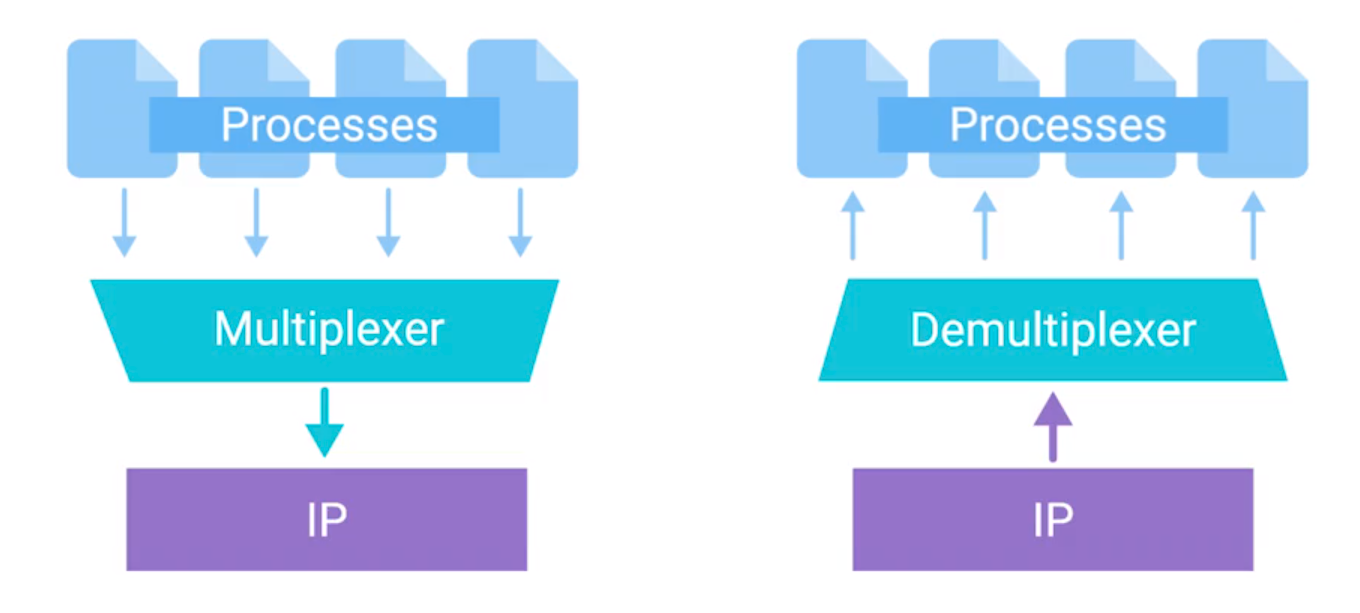
\includegraphics[width=0.6\textwidth]{figures/Multiplexing Demultiplexing.png}
\end{figure}

\section{Encapsulation and Decapsulation}
Encapsulation is the process of adding header and trailer information to a data packet at each layer of the OSI model, while decapsulation is the reverse process of removing these headers and trailers at the receiving end. This structured approach ensures data transmission and reception across a network.

\begin{figure}[H]
   \centering
   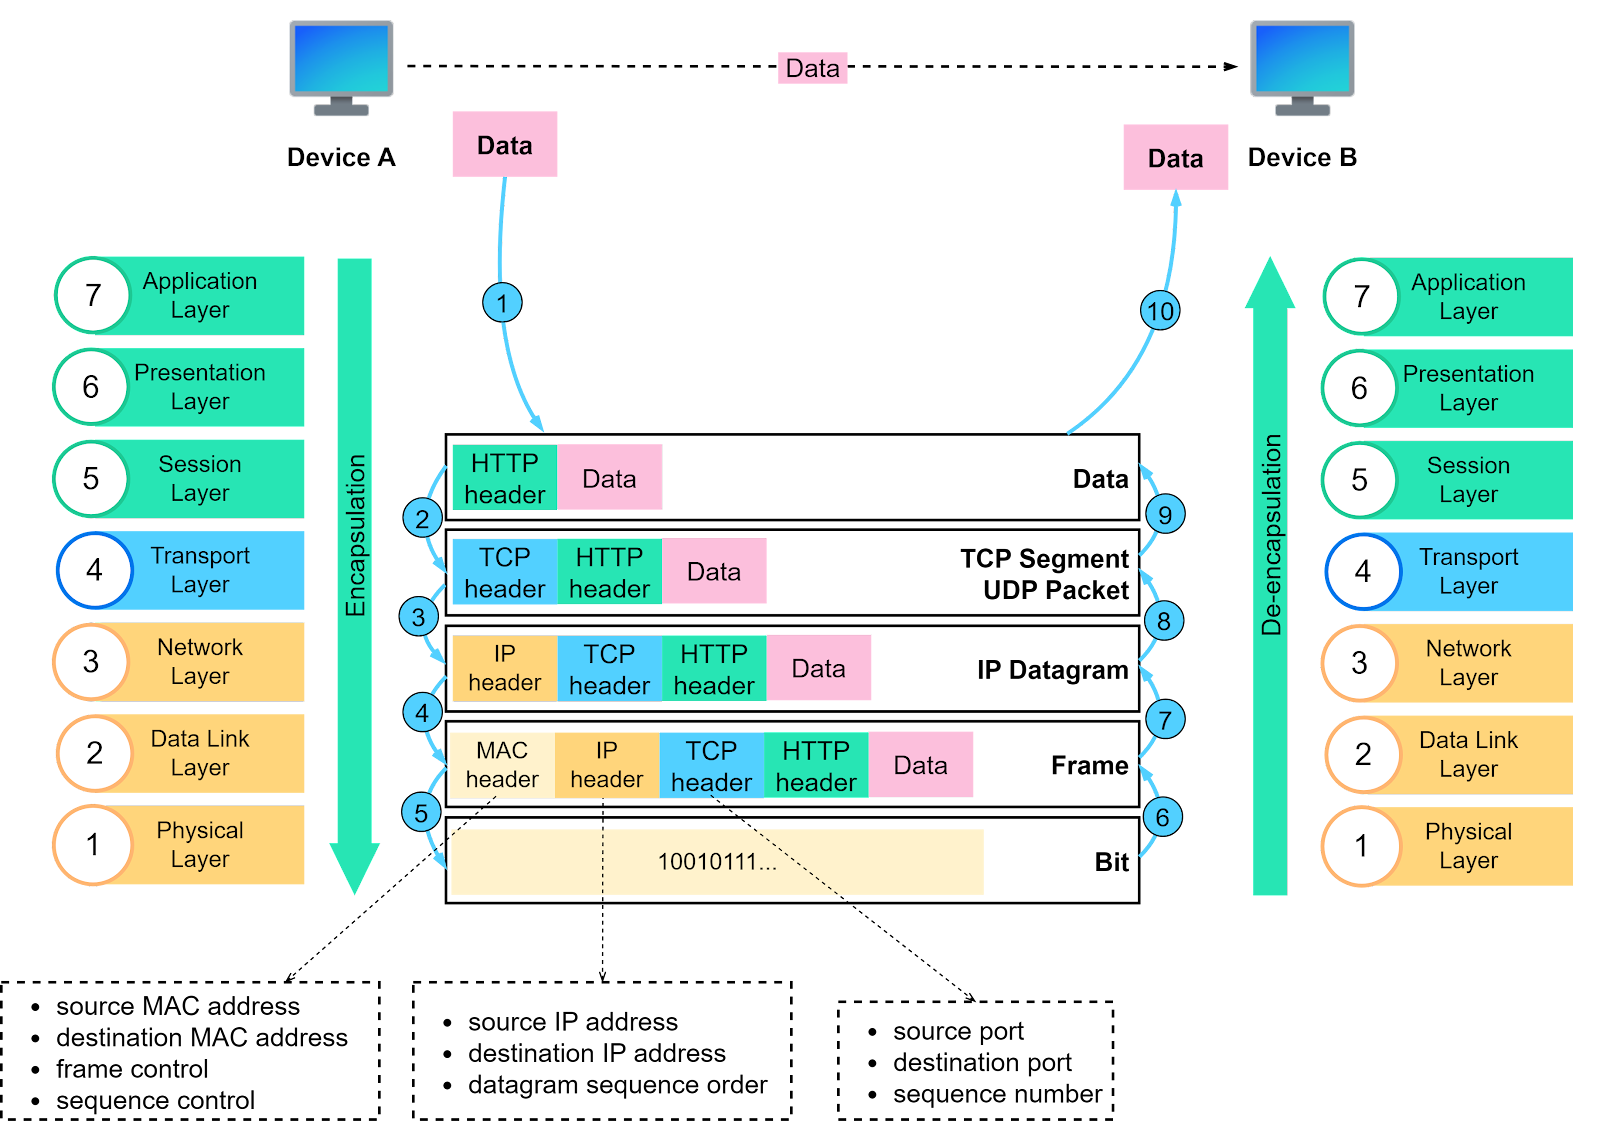
\includegraphics[width=0.6\textwidth]{figures/Capsulation.png}
\end{figure}

\section{TCP and UDP}

\begin{tabularx}{\textwidth}{|X|X|}\hline
   \thc{Transmission Control Protocol(TCP)} & \thc{User Datagram Protocol (UDP)}\\\hline
   connection oriented protocol & connectionless protocol \\\hline
   reliable & not reliable \\\hline
   slower & faster \\\hline
   An acknowledgment segment is present & No acknowledgment segment \\\hline
   possible retransmission & no retransmission \\\hline
   20-60 bytes variable length header & 8 bytes fixed length header \\\hline
\end{tabularx}

\begin{figure}[H]
   \centering
   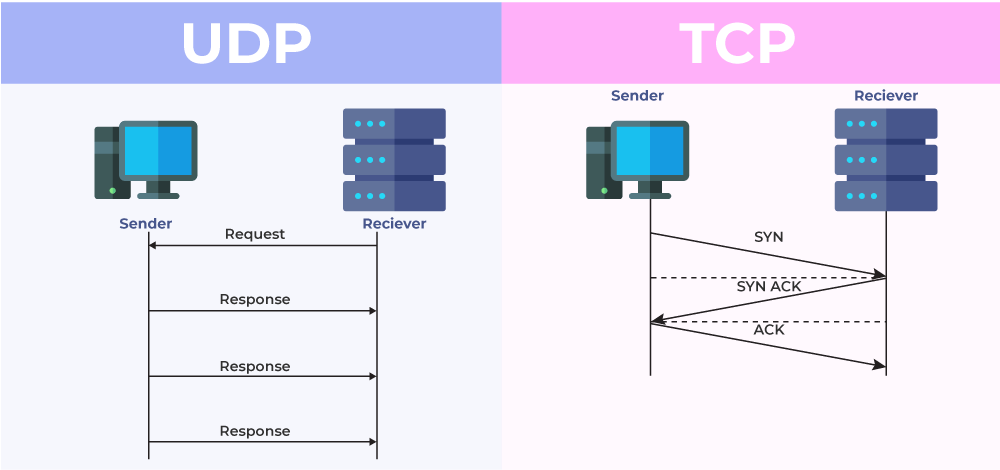
\includegraphics[width=0.6\textwidth]{figures/TCP and UDP.png}
\end{figure}

\vspace{1em}
\section{SSL and TLS}
SSL (Secure Sockets Layer) and TLS (Transport Layer Security) are cryptographic protocols designed to provide secure communication over a network. SSL was the original protocol developed by Netscape, but it has known vulnerabilities and is now considered obsolete.

TLS is the modern, more secure successor to SSL. It offers better encryption algorithms, improved key exchange mechanisms, and stronger message authentication. TLS ensures confidentiality, integrity, and authentication in data transmission, and is widely used in securing web traffic (HTTPS), emails, and VoIP.

\vspace{1em}
\section{Practice Problems}
\begin{enumerate}
   \item \textbf{TCP Throughput Calculation}
   \begin{itemize}
       \item \textbf{Question:} A TCP connection has a window size of 65,535 bytes and a round-trip time (RTT) of 100 ms. What is the maximum achievable throughput?
       \item \textbf{Solution:} 
       \begin{align*}
           \text{Throughput} &= \frac{\text{Window Size}}{\text{RTT}} \\
           &= \frac{65535 \text{ bytes}}{0.1 \text{ sec}} \\
           &= 655,350 \text{ bytes/sec} \approx 655.35 \text{ KBps}
       \end{align*}
   \end{itemize}

   \pagebreak
   \item \textbf{UDP vs TCP Header Overhead}
   \begin{itemize}
       \item \textbf{Question:} If you send a 1000-byte message using TCP and UDP, what is the actual data size transmitted (including headers)?
       \item \textbf{Solution:}
       \begin{itemize}
           \item \textbf{TCP:} Header = 20 bytes, IP Header = 20 bytes \\
           Total = 1000 + 20 + 20 = 1040 bytes
           \item \textbf{UDP:} Header = 8 bytes, IP Header = 20 bytes \\
           Total = 1000 + 8 + 20 = 1028 bytes
       \end{itemize}
   \end{itemize}

   \item \textbf{Segment Count for a File}
   \begin{itemize}
       \item \textbf{Question:} A file of size 10 MB is being sent using TCP, with each segment carrying 1460 bytes of data. How many segments are needed?
       \item \textbf{Solution:}
       \begin{align*}
           \text{Segments} &= \left\lceil\frac{10 \times 1024 \times 1024}{1460}\right\rceil \\
           &= \left\lceil\frac{10485760}{1460}\right\rceil \\
           &= 7184 \text{ segments}
       \end{align*}
   \end{itemize}

   \item \textbf{Round-Trip Delay and Acknowledgment}
   \begin{itemize}
       \item \textbf{Question:} A sender is transmitting packets of 1000 bytes over a TCP connection. The RTT is 200 ms, and the receiver sends an acknowledgment every 2 packets. What is the average data rate?
       \item \textbf{Solution:}
       \begin{itemize}
           \item Total data acknowledged per RTT = 2 × 1000 = 2000 bytes
           \item RTT = 0.2 sec
       \end{itemize}
       \begin{align*}
           \text{Throughput} &= \frac{2000}{0.2} \\
           &= 10,000 \text{ bytes/sec} \\
           &= 10 \text{ KBps}
       \end{align*}
   \end{itemize}
\end{enumerate}